\documentclass[12pt]{article}
\usepackage[utf8]{inputenc}
\usepackage{listings}
\usepackage{xcolor}
\usepackage{graphicx}
\graphicspath{ {./images/} }
%To embed code

\lstset{frame=tb,
  language=c++,
  aboveskip=3mm,
  belowskip=3mm,
  showstringspaces=false,
  columns=flexible,
  basicstyle={\small\ttfamily},
  numbers=none,
  numberstyle=\tiny\color{gray},
  keywordstyle=\color{blue},
  commentstyle=\color{dkgreen},
  stringstyle=\color{mauve},
  breaklines=true,
  breakatwhitespace=true,
  tabsize=3
}

\title{Analysis and Design of Algorithms}
\author{Fernando Socualaya}
\date{April 2019}

\usepackage{natbib}
\usepackage{graphicx}
\usepackage{hyperref}

\begin{document}

\maketitle

\section{Warm up}

% Explanation of modified 3 - way merge sort

As its known Merge Sort is a Divide and Conquer algorithm, it works dividing the array to be sorted into two halves until get a single array and then sorting and merging the single arrays. In order to calculate the complexity of the algorithm splitting the given array in three parts instead of two halves we have to consider that, being $x$ the number of times that we have to split the array, and $n$ the number of elements in the array, then $2^x = n$ or $x = \log_2 n$. Multiplying it by the size of the initial array, we get that the complexity of Merge Sort is $O(n\log_2 n)$. In that way, if we try to split in three parts instead of two halves the algorithm's complexity will be given by $n3^x = n$ or $n\log_3 n$.  

\section{Competitive programming}

\begin{itemize}
    \item \textbf{100 - 3n + 1}
    
    \begin{lstlisting}
#include <iostream>
#include <fstream>
using namespace std;

int tresenemasuno(long int n){
    int count = 1;

    if (n == 0){
        return n;
    }

    while(n!=1){
        if(!(n%2))
            n /= 2;
        else
            n = 3*n+1;
        ++count;
    }
    return count;
};

int getMax(int start, int end){
	int max = tresenemasuno(start);
	for(int i=start;i<=end;i++){
		if(tresenemasuno(i)>max)
			max = tresenemasuno(i);
	}
	return max;
};

int main(){
    	int start=0, end=0;
	while(cin>>start>>end){		
		cout<<start<<' '<<end<<' ';
		if(start>end) cout<<getMax(end,start);
		else cout<<getMax(start,end);
		cout<<'\n';
	}
	return 0;
}
    \end{lstlisting}
    
    \item \textbf{458 - The Decoder}
    
    \begin{lstlisting}
#include <iostream>
using namespace std;

int main(){
	string encoded;
	while(cin>>encoded){
		for(auto&i:encoded)
			cout<<(char)(i-7);
		
		cout<<endl;
	}
	return 0;	
}
    \end{lstlisting}
    
\end{itemize}

\section{Simulation}

\begin{itemize}
    \item Insertion sort algorithm: Implemented at $"sortingAlgorithms.h"$
    
    \begin{lstlisting}
    void insertionSort(int a[], int size){
        for(int j=1;j<size;j++){
            int key = a[j];
            int i = j-1;
            while(i>=0 and a[i]>key){
                a[i+1] = a[i];
                i--;
            }
            a[i+1] = key;
        }
    \end{lstlisting}

    \item Merge sort algorithm: $"sortingAlgorithms.h"$
    
    \begin{lstlisting}
    void Merge(int A[], int p, int q, int r){
        //Sizes for new arrays
        int n1 = q-p+1;
        int n2 = r-q;
    
        //let L[1 ... n1 + 1] and R[1 ... n2 + 1] be new arrays
        int L[n1+1]={};
        int R[n2+1]={};
        for(int i = 0;i<n1;i++) L[i] = A[p+i];
        for(int j = 0;j<n2;j++) R[j] = A[q+j+1];
    
        L[n1] = std::numeric_limits<int>::max();
        R[n2] = std::numeric_limits<int>::max();
    
        int i = 0;
        int j = 0;
    
        for(int k = p; k<=r; k++){
            if(L[i]<=R[j]){
                A[k] = L[i];
                i++;
            }
            else{
                A[k] = R[j];
                j++;
            }
        }
    };

    void MergeSort(int A[], int p, int r){
        if(p<r){
            int q = floor((float)(p+r)/2);
            MergeSort(A,p,q);
            MergeSort(A,q+1,r);
            Merge(A,p,q,r);
        }
    };
    \end{lstlisting}
    
    \item Simulations: To run the simulations was implemented a C++ program(\textbf{simulation.cpp})to write the sizes and its respective average running time(for both algorithms) into the $simulation.csv$ file. This program receive three numbers as input, the starting size, the limit size, and the number of times runned to get the average. The results obtained were plotted using the \textbf{matplotlib} library on python. As it can be seen in $Figure 1$, \textbf{Merge Sort}($O(nlog(n))$) algorithm grow slower than \textbf{Insertion Sort}($O(n^2)$). However, at the beginning insertion sort grows slower than merge sort, this happens until the cut point of both curves, henceforth, the polynomial growth of insertion sort is evident in comparison to the logarithmic growth of merge sort.
    
    \begin{figure}[htbp]
        \centering
        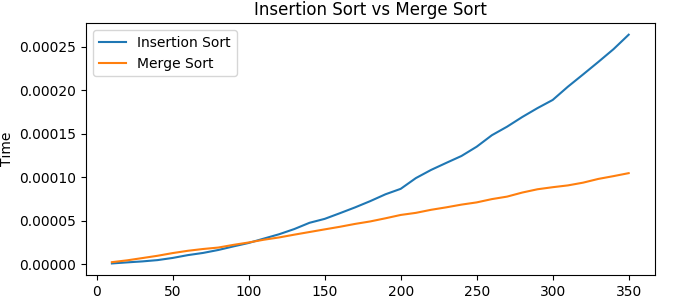
\includegraphics[width=0.7\textwidth]{Semana2_Entrega/images/Sorting_Algorithms.png}
        \caption{Algorithms Running Time Comparison}
        \label{fig:my_label}
    \end{figure}
\end{itemize}

\emph{Note:} All algorithms are placed in the /3\_Simulation folder.

\section{Research}

% Karatsuba? :c 

\section{Wrapping up}

After comparing the complexity(Figure 2), is evident the fast growth of some ones respect others. In detail and ordered by growth:

\begin{figure}[!htbp]
    \centering
    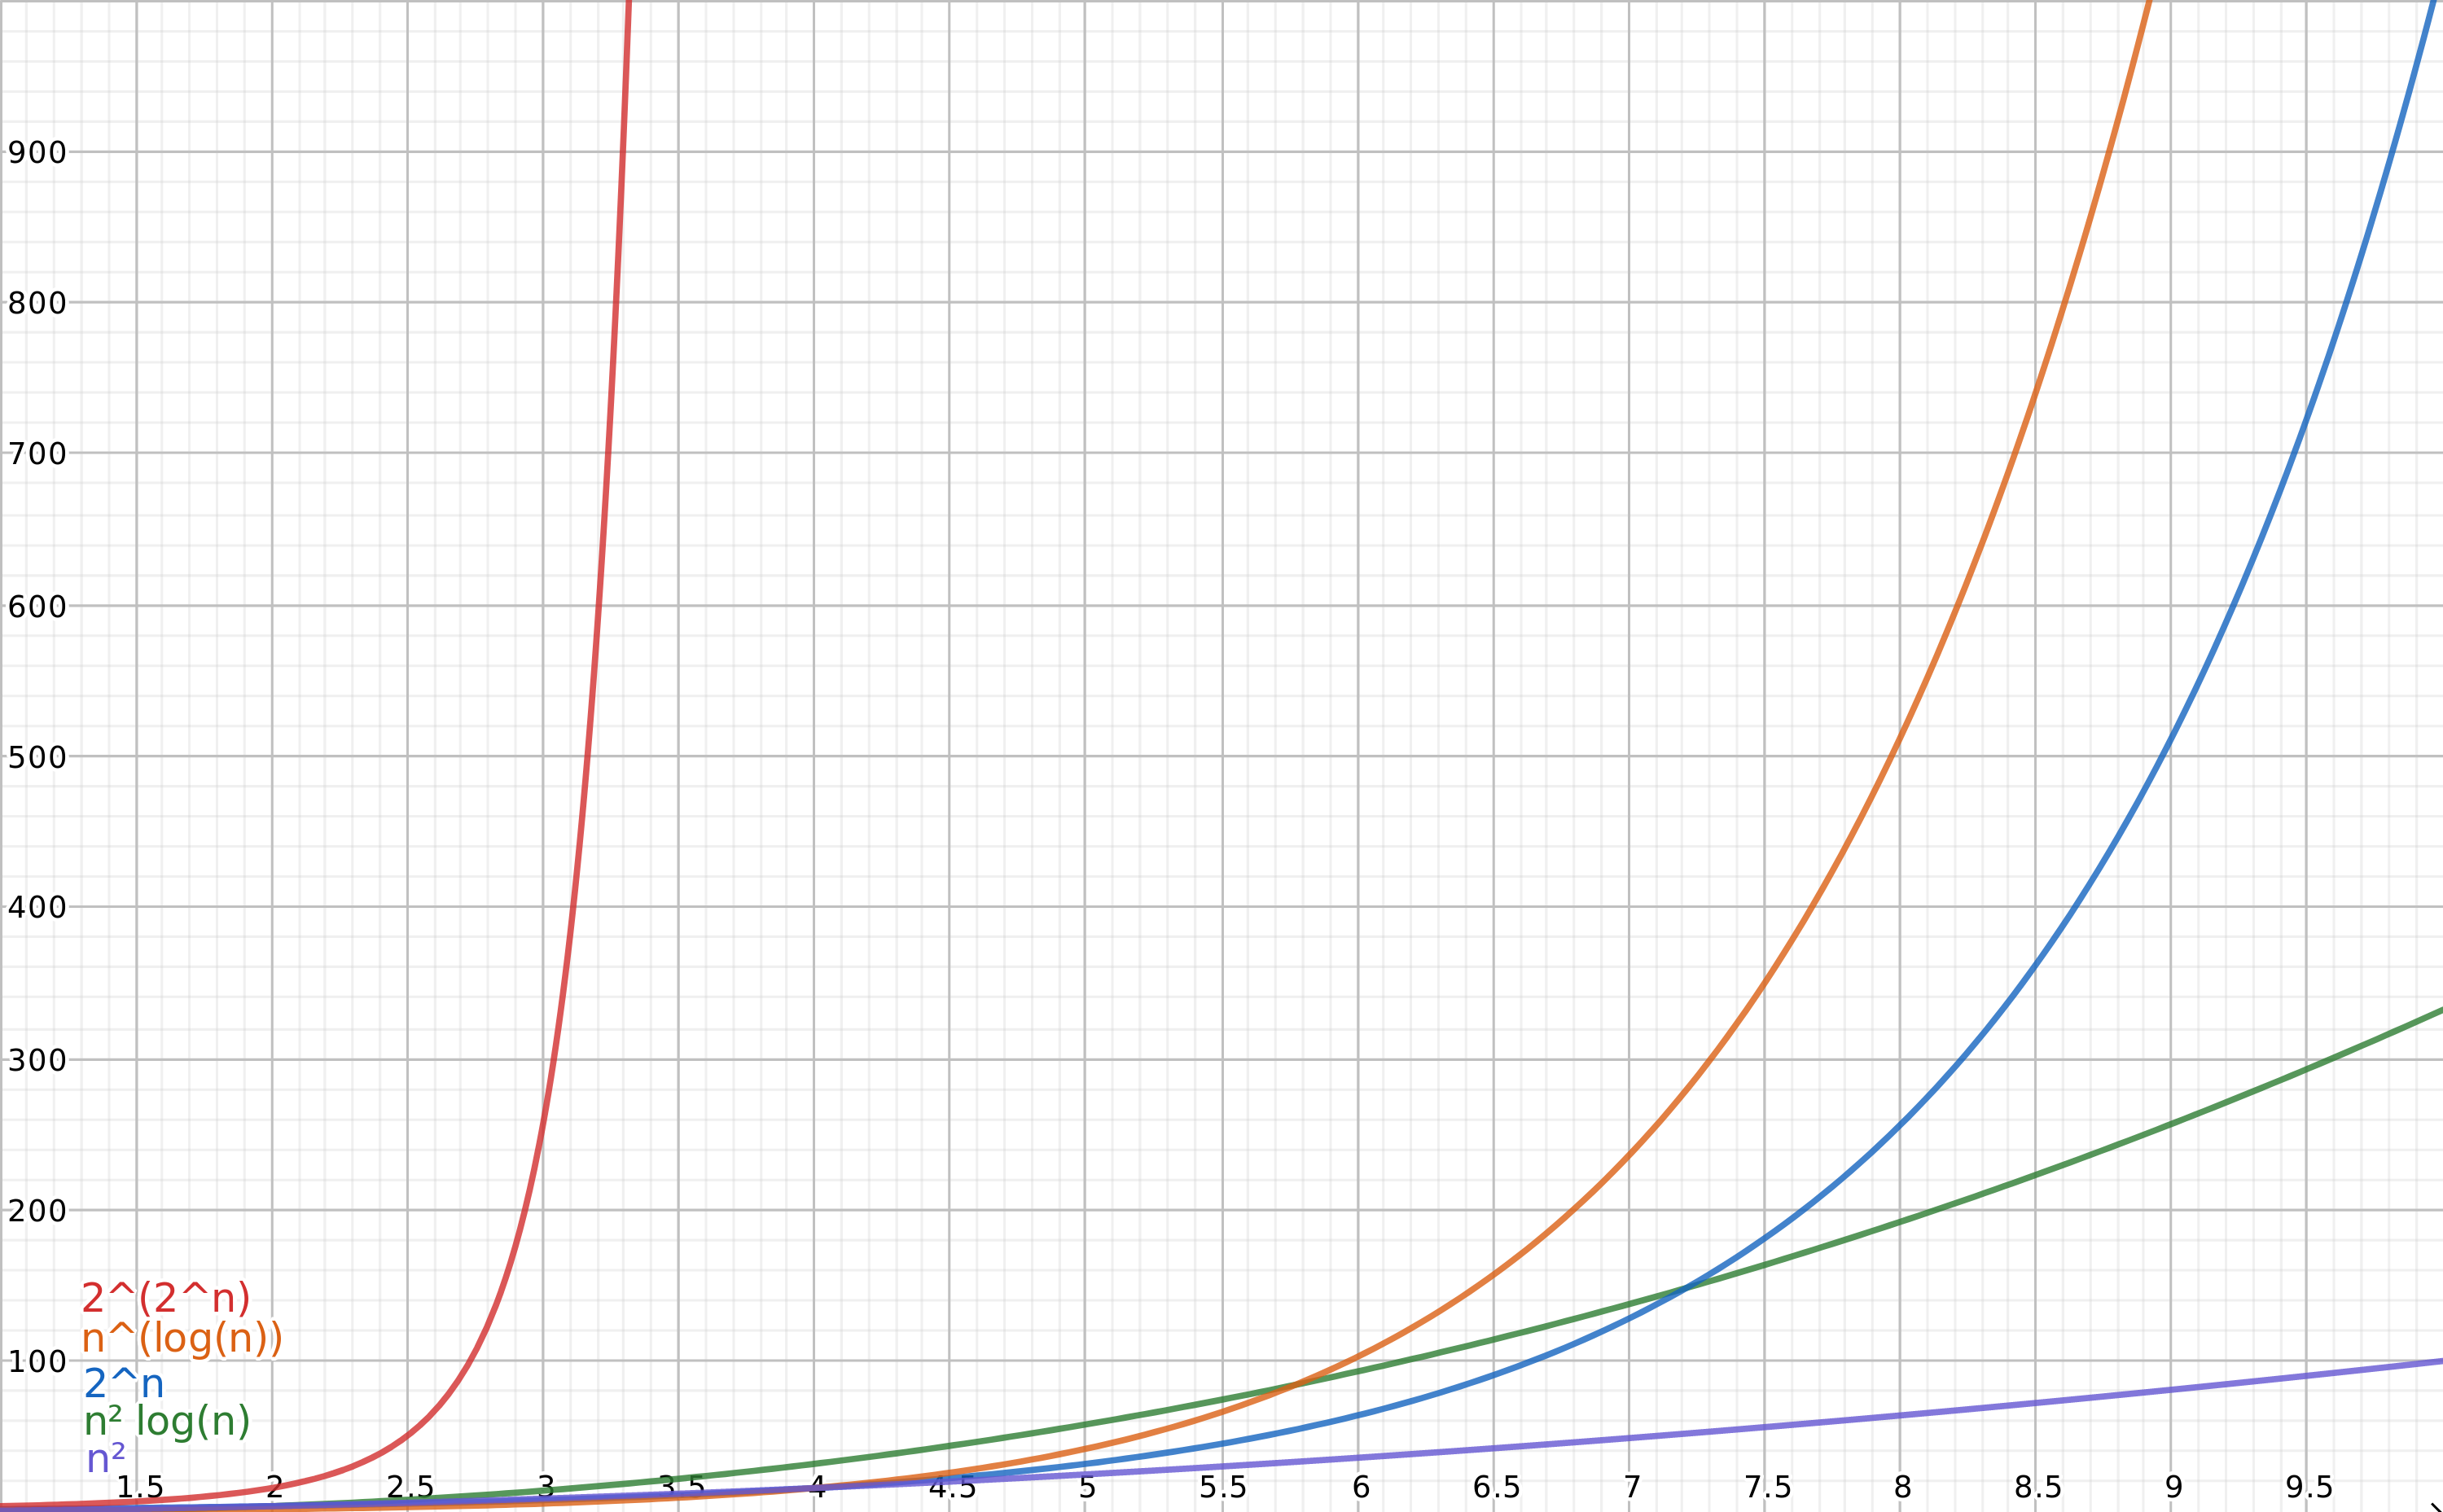
\includegraphics{Semana2_Entrega/images/complexity_analysis.png}
    \caption{Algorithm complexity}
    \label{fig:my_label}
\end{figure}


\begin{enumerate}
    \item $n^{2}$: With small values grows fast. However, it grows slower than the other ones as $n$ grows. It ended being the slowest-growth complexity.
    \item $n^{2}log(n)$: Started being the slowest-growth complexity. With small values growth faster than the others, but with high values it became the second fast-growth complexity.
    \item $2^{n}$: Started being the second fast-growth complexity, but after cutting $n^{2}log(n)$ and $n^{2}$ first, and then $n^{2}$(one more time) and $n^{log(n)}$. It ended in the third position. 
    \item $n^{log(n)}$: Looks like a slow-growth complexity with small values, however, as they grow, its growth turns faster. End being the second fast-growth complexity.
    \item $2^{2^{n}}$: Fast growth, it reaches high f(n) values with small n. Ended being the faster-growth complexity.
     
\end{enumerate}

\end{document}
